\documentclass[a4paper, 11pt]{article}
\usepackage{comment} % enables the use of multi-line comments (\ifx \fi) 
\usepackage{fullpage} % changes the margin
\usepackage{amsmath}
\usepackage[makeroom]{cancel}

\usepackage{graphicx}
\usepackage[]{textcomp}

\usepackage{geometry}
 \geometry{
 a4paper,
 left=15mm,
 right=15mm,
 top=15mm,
 }

\begin{document}

\noindent 
\includegraphics[scale=0.2]{figures/logo.png}\\
\large\textbf{Projet de semestre - C\raisebox{.5\height}{\scalebox{.5}{++}} orienté objet} \hfill \textbf{Rafael RIBER  - SCIPER: 296142} \\
\large\textbf{Dodgeball} \hfill \hfill \textbf{Valentin RIAT - SCIPER: 289121}\\
\normalsize COM-112(a) \hfill \textbf{EL-BA2 - Semestre de printemps 2018-2019}
\section{Architecture logicielle et description de l’implémentation:}

\subsection{Structuration des données}

L'ensemble des joueurs (chacun une instance de la classe \texttt{Player}) est stocké dans un \texttt{vector} appelé \texttt{players}, attribut de la classe \texttt{Simulation}. Les balles sont stockées de manière identique dans un \texttt{vector} appelé \texttt{balls}.

La carte est est stockée comme une instance de la classe \texttt{Map}, attribut de la simulation. Au sein de \texttt{Map}, le \texttt{vector} 2D \texttt{obstacleMap} stocke les cases où un obstacle est présent, représentées par '\texttt{1}', et les cases libres, représentées par '\texttt{0}'.

\subsection{Répartition des tâches entre les modules}

À chaque mise à jour, on appele la fonction \texttt{simulate\_one\_step()} de \texttt{Simulation}. Cette fonction, par des sous-fonctions, détermine la cible de chaque joueur, et assigne l'addresse de la cible à l'attribut \texttt{target} des joueurs. 

Elle déplace ensuite chaque joueur vers sa cible, et crée ensuite des nouvelles instances de \texttt{Ball} si des balles sont tirées, et les fait bouger selon leur trajectoire. 
Les tests de collision balle-joueur, balle-obstacle et balle-balle sont effectués au sein du module simulation, qui modifie les structures de données en conséquence. Le module simulation s'occupe ainsi du stockage et de l'intéraction des éléments de jeu. Les détails d'implémentation et les attributs de ces éléments de jeu sont traités par les modules correspondants (\texttt{Ball}, \texttt{Player} et \texttt{Map}).

La matrice des distances est calculée pour la première fois à la lecture du fichier, et est recalculée lorsqu'un obstacle est éliminé par une balle.

\subsection{Coût calcul et coût mémoire}

Dans le pire des cas, à savoir quand un obstacle est éliminé et on recalcule la matrice des distances, le coût calcul d'une mise a jour est d'ordre $\mathcal{O}(\text{nbSpot}^3)$. 

La matrice des distances est de taille $\text{nbSpot}^2$. Comme on a $\text{nbSpot} = \text{nbCell}^2 - \text{nbObst}$, le coût mémoire d'une mise a jour est donc d'ordre $\mathcal{O}(\text{nbCell}^4)$.

\subsection{Exemple de simulation}
(Les images sont parfois séparées de plusieurs mises à jour)\\
\begin{minipage}{0.33333333\textwidth}
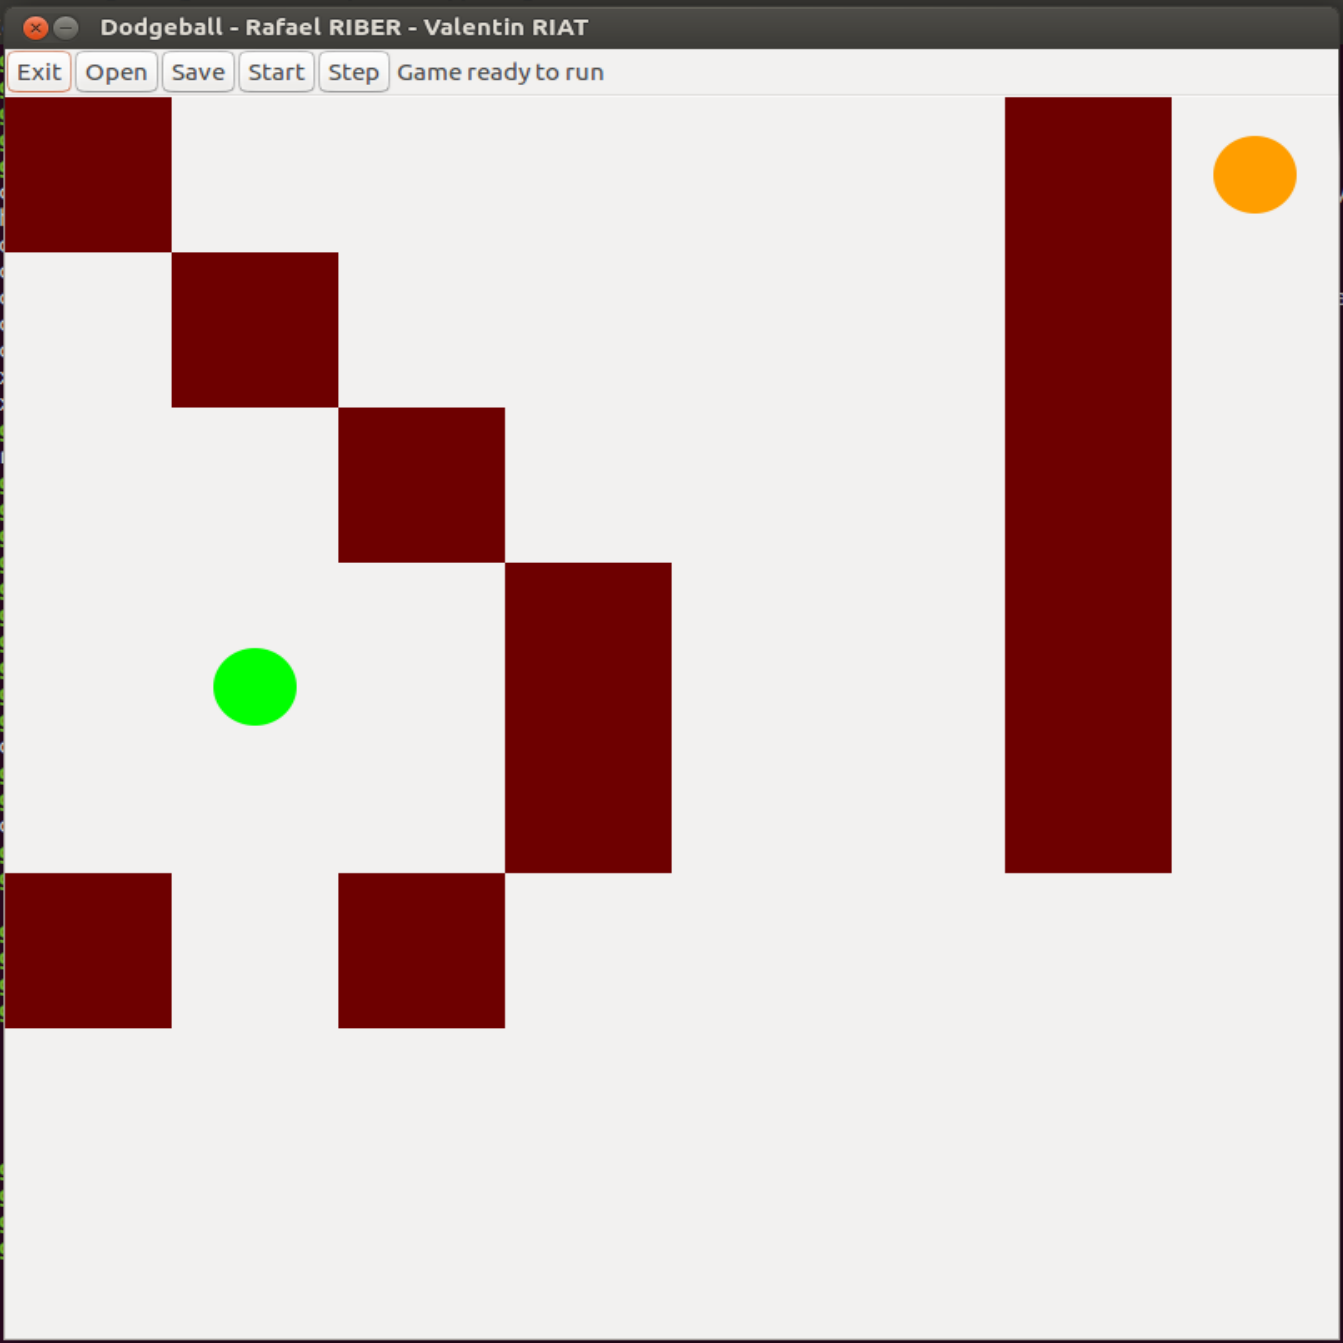
\includegraphics[width=\textwidth]{figures/sim1.PNG}
\end{minipage}
\begin{minipage}{0.33333333\textwidth}
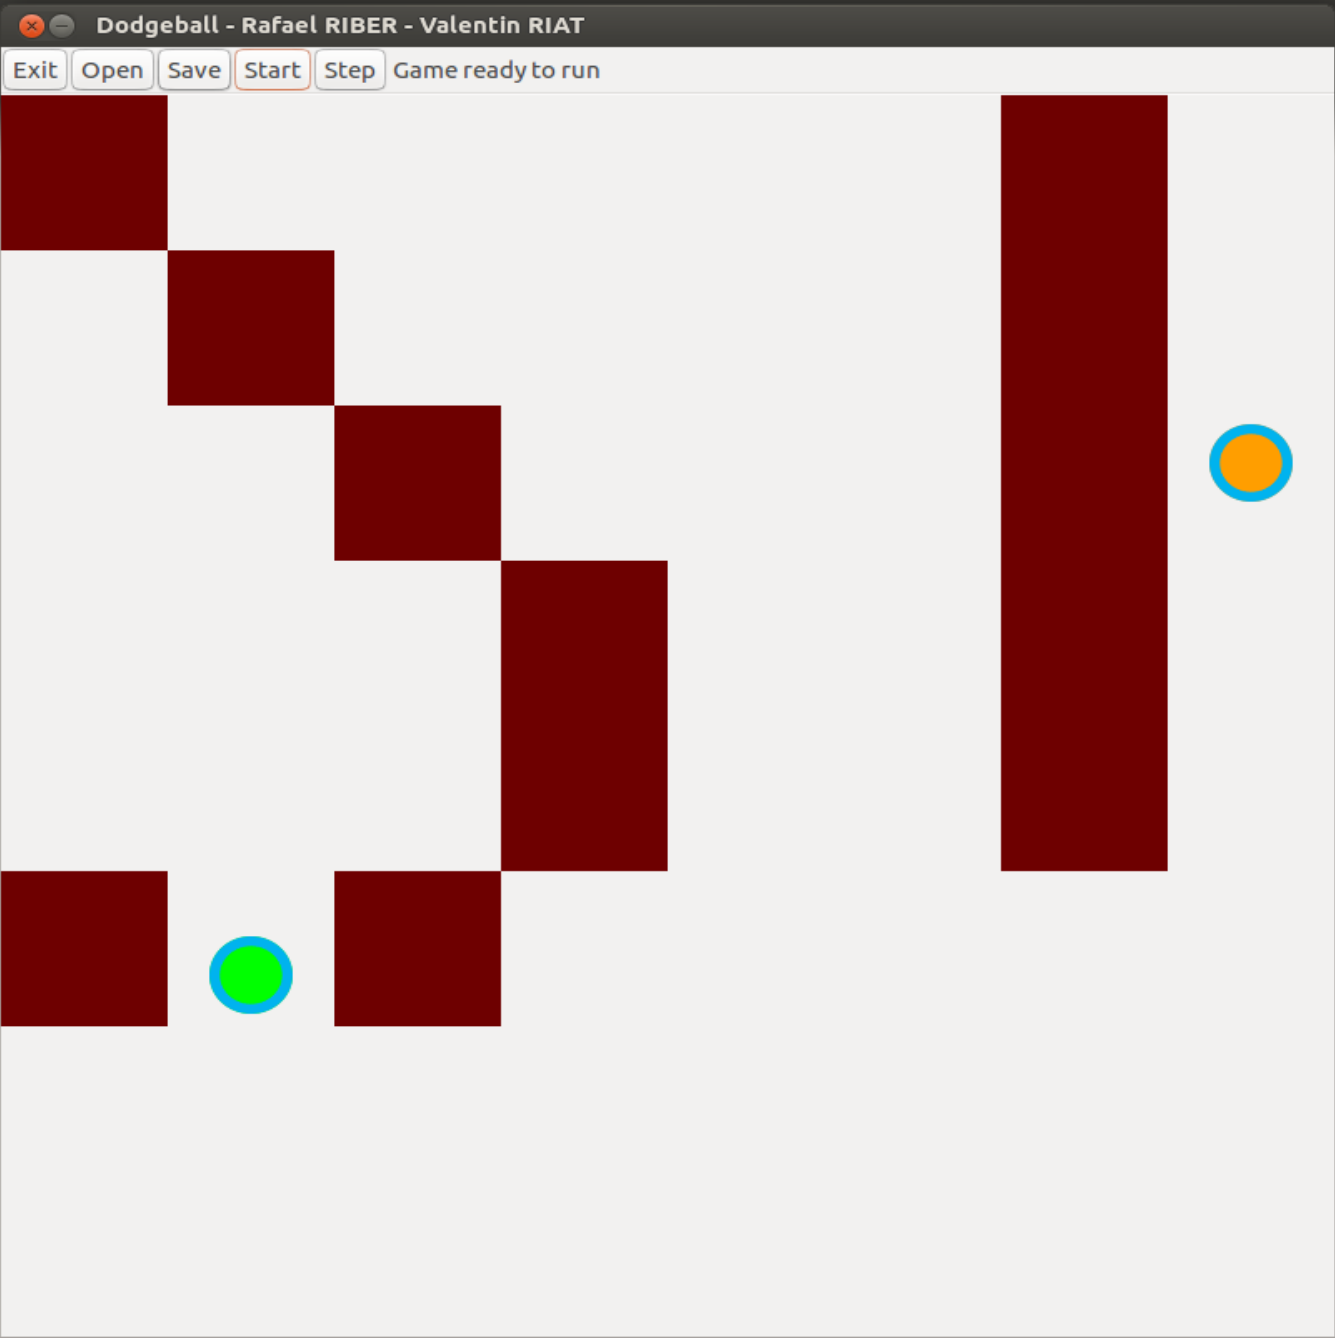
\includegraphics[width=\textwidth]{figures/sim2.PNG}
\end{minipage}
\begin{minipage}{0.33333333\textwidth}
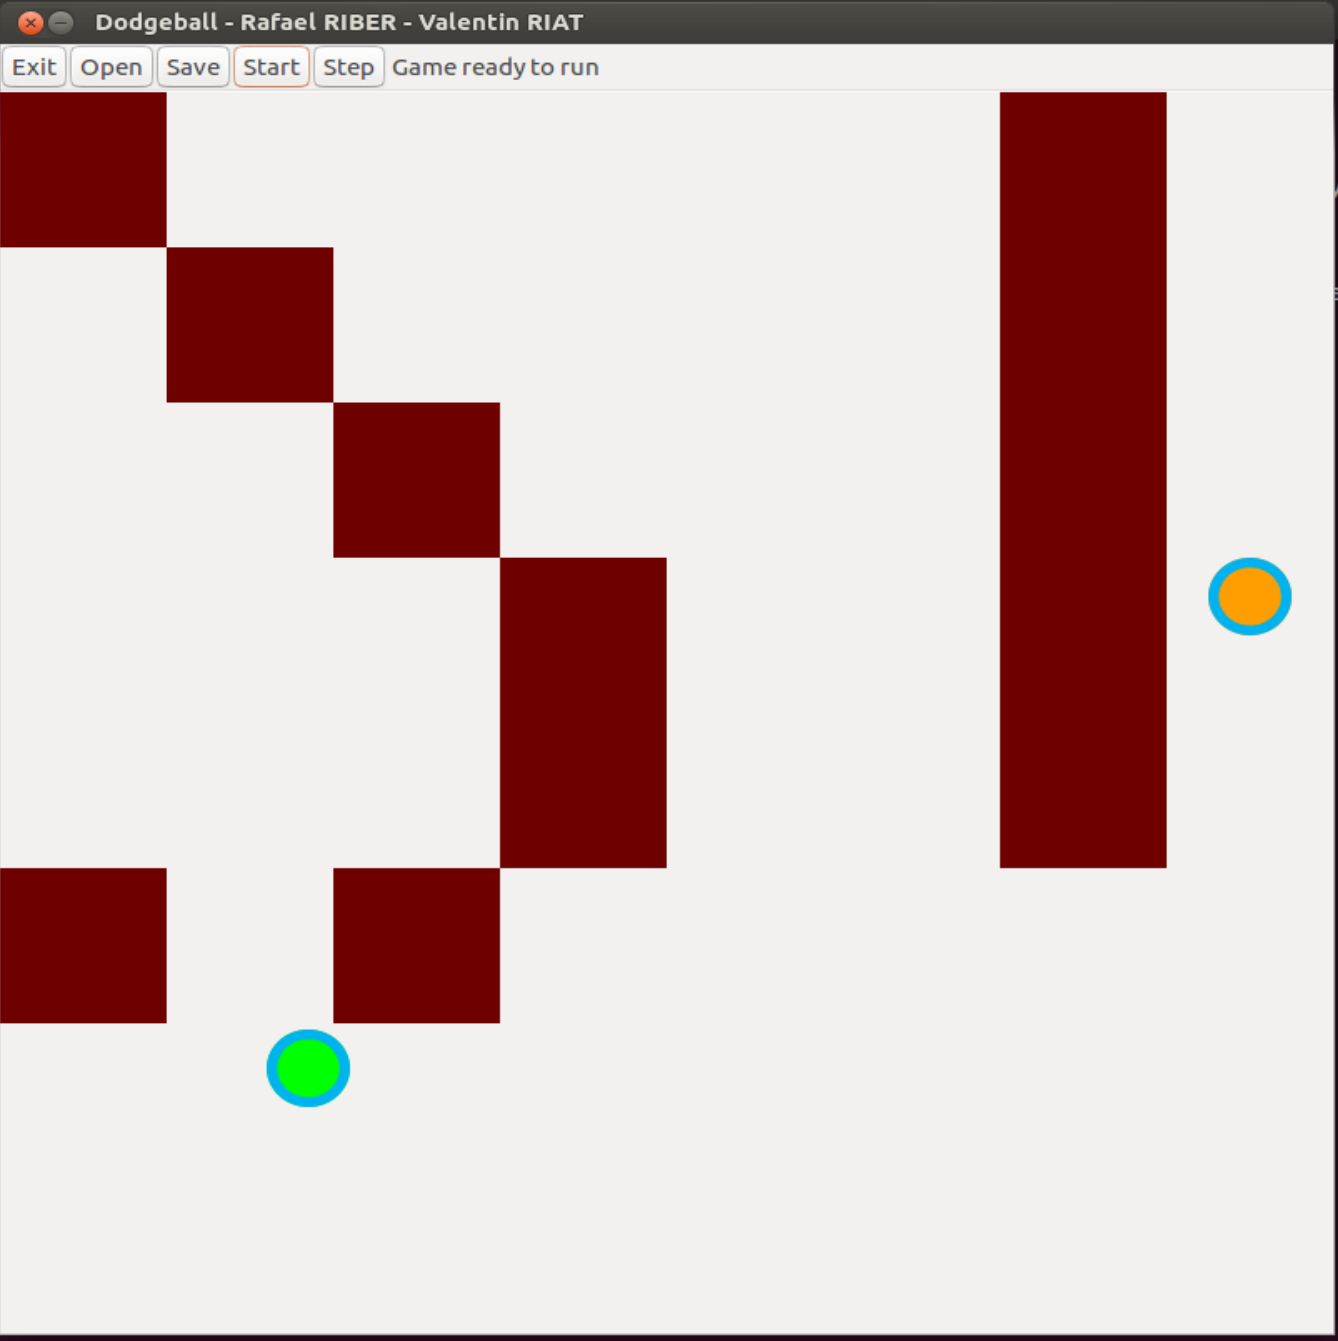
\includegraphics[width=\textwidth]{figures/sim3.PNG}
\end{minipage}\\
\begin{minipage}{0.33333333\textwidth}
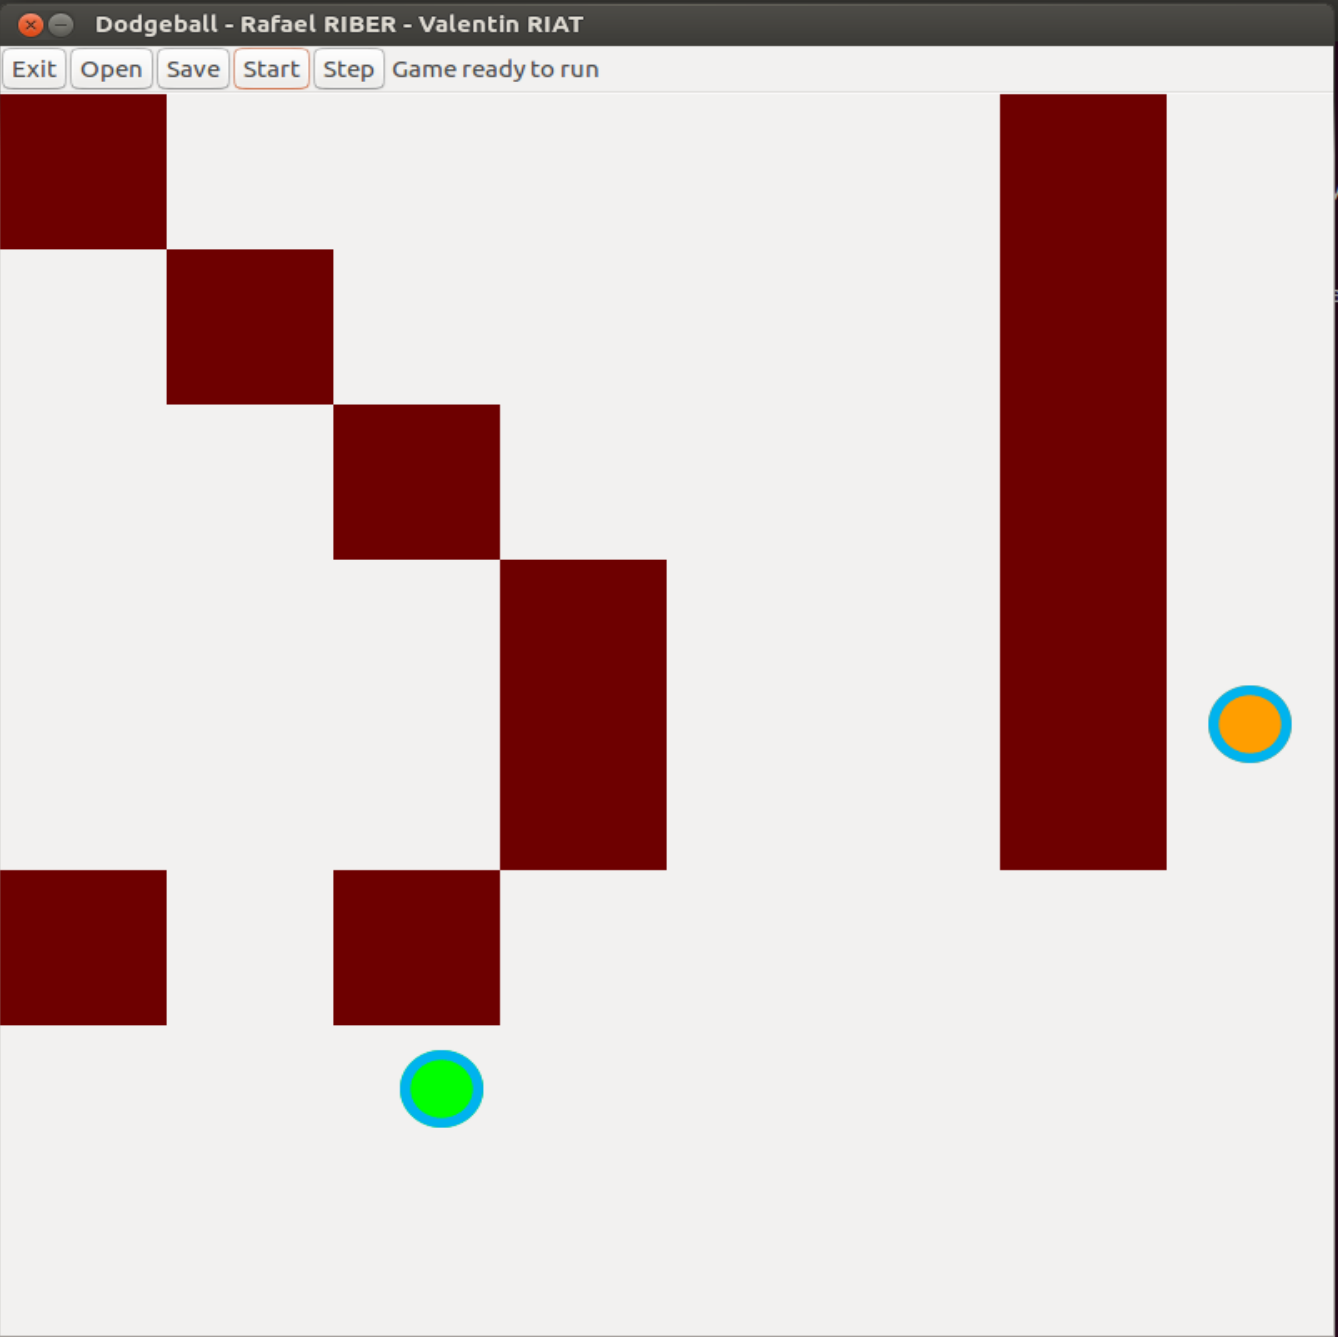
\includegraphics[width=\textwidth]{figures/sim4.PNG}
\end{minipage}
\begin{minipage}{0.33333333\textwidth}
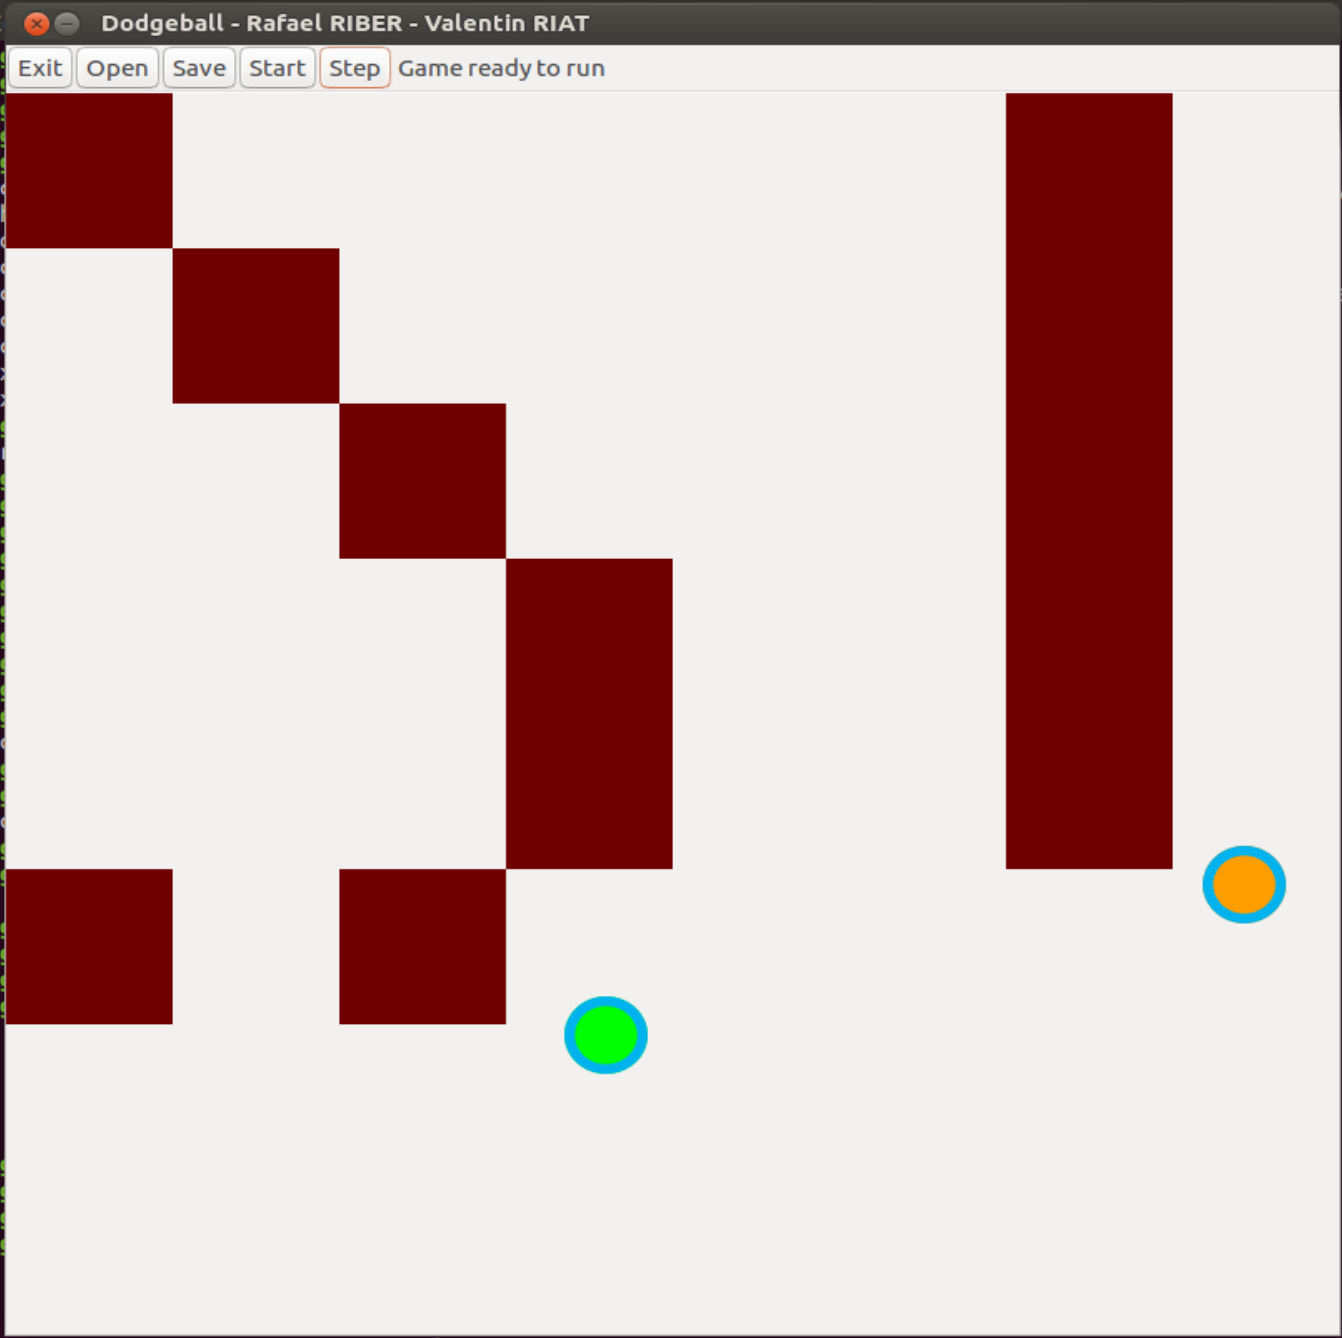
\includegraphics[width=\textwidth]{figures/sim6.PNG}
\end{minipage}
\begin{minipage}{0.33333333\textwidth}
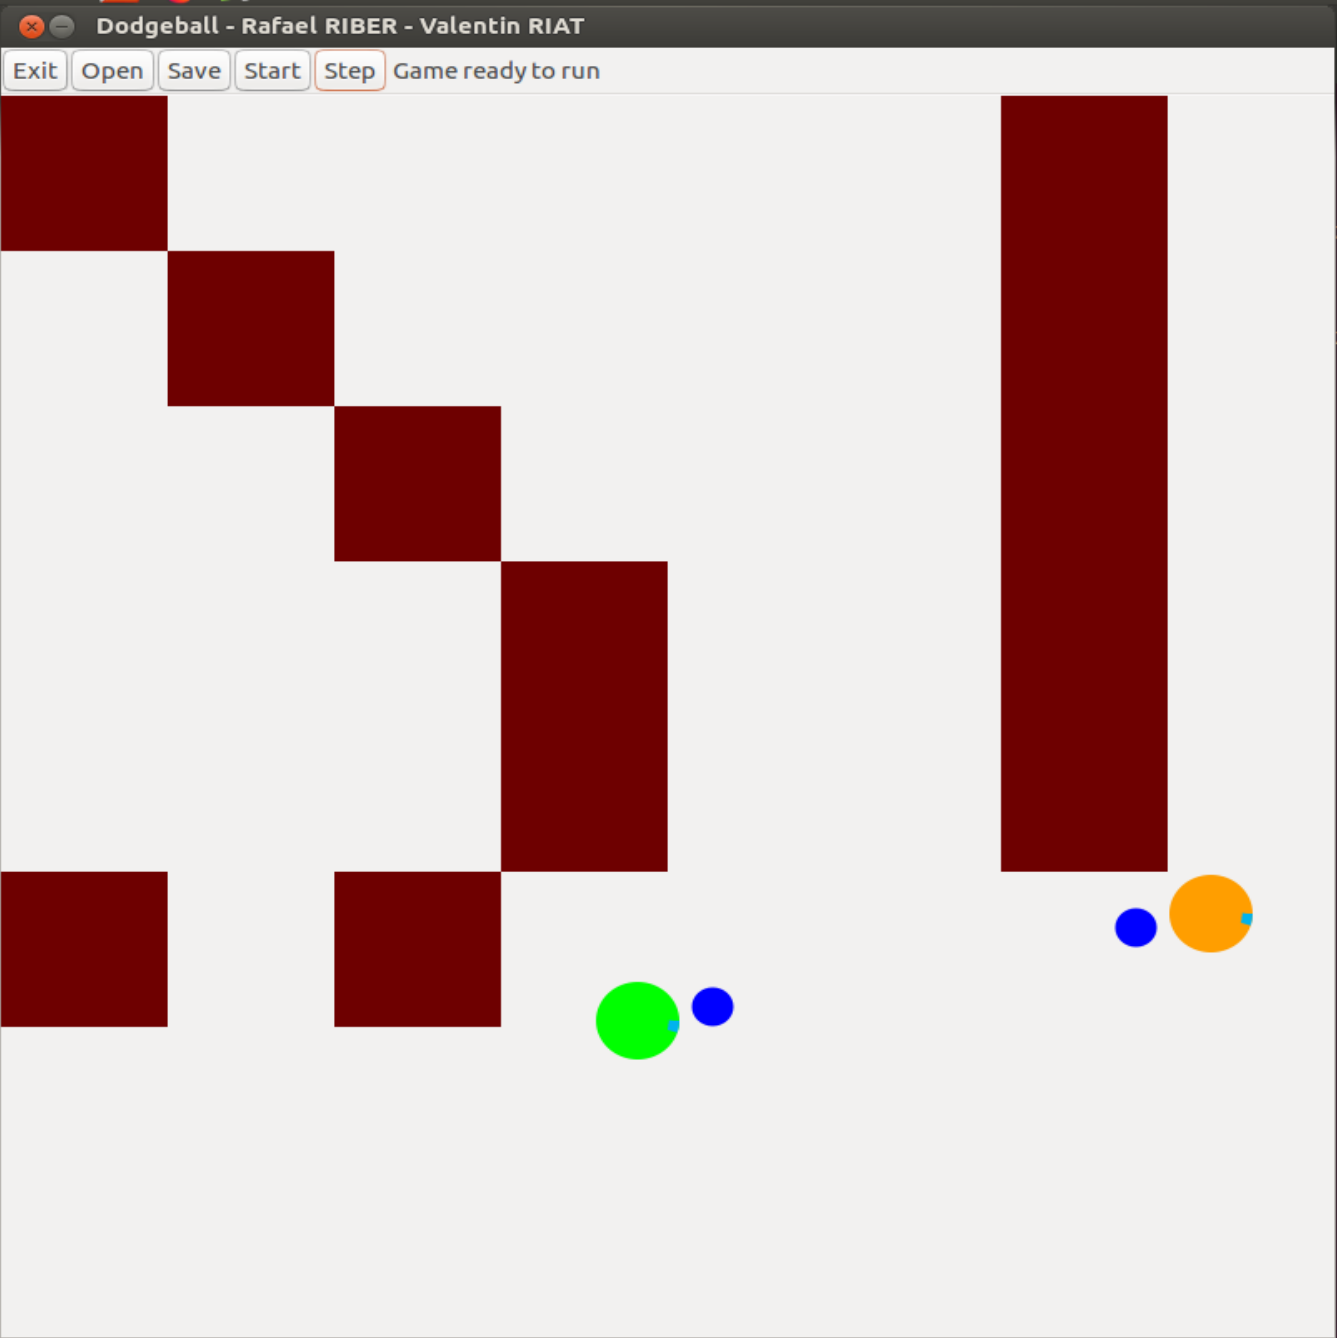
\includegraphics[width=\textwidth]{figures/sim7.PNG}
\end{minipage}\\
\begin{minipage}{0.33333333\textwidth}
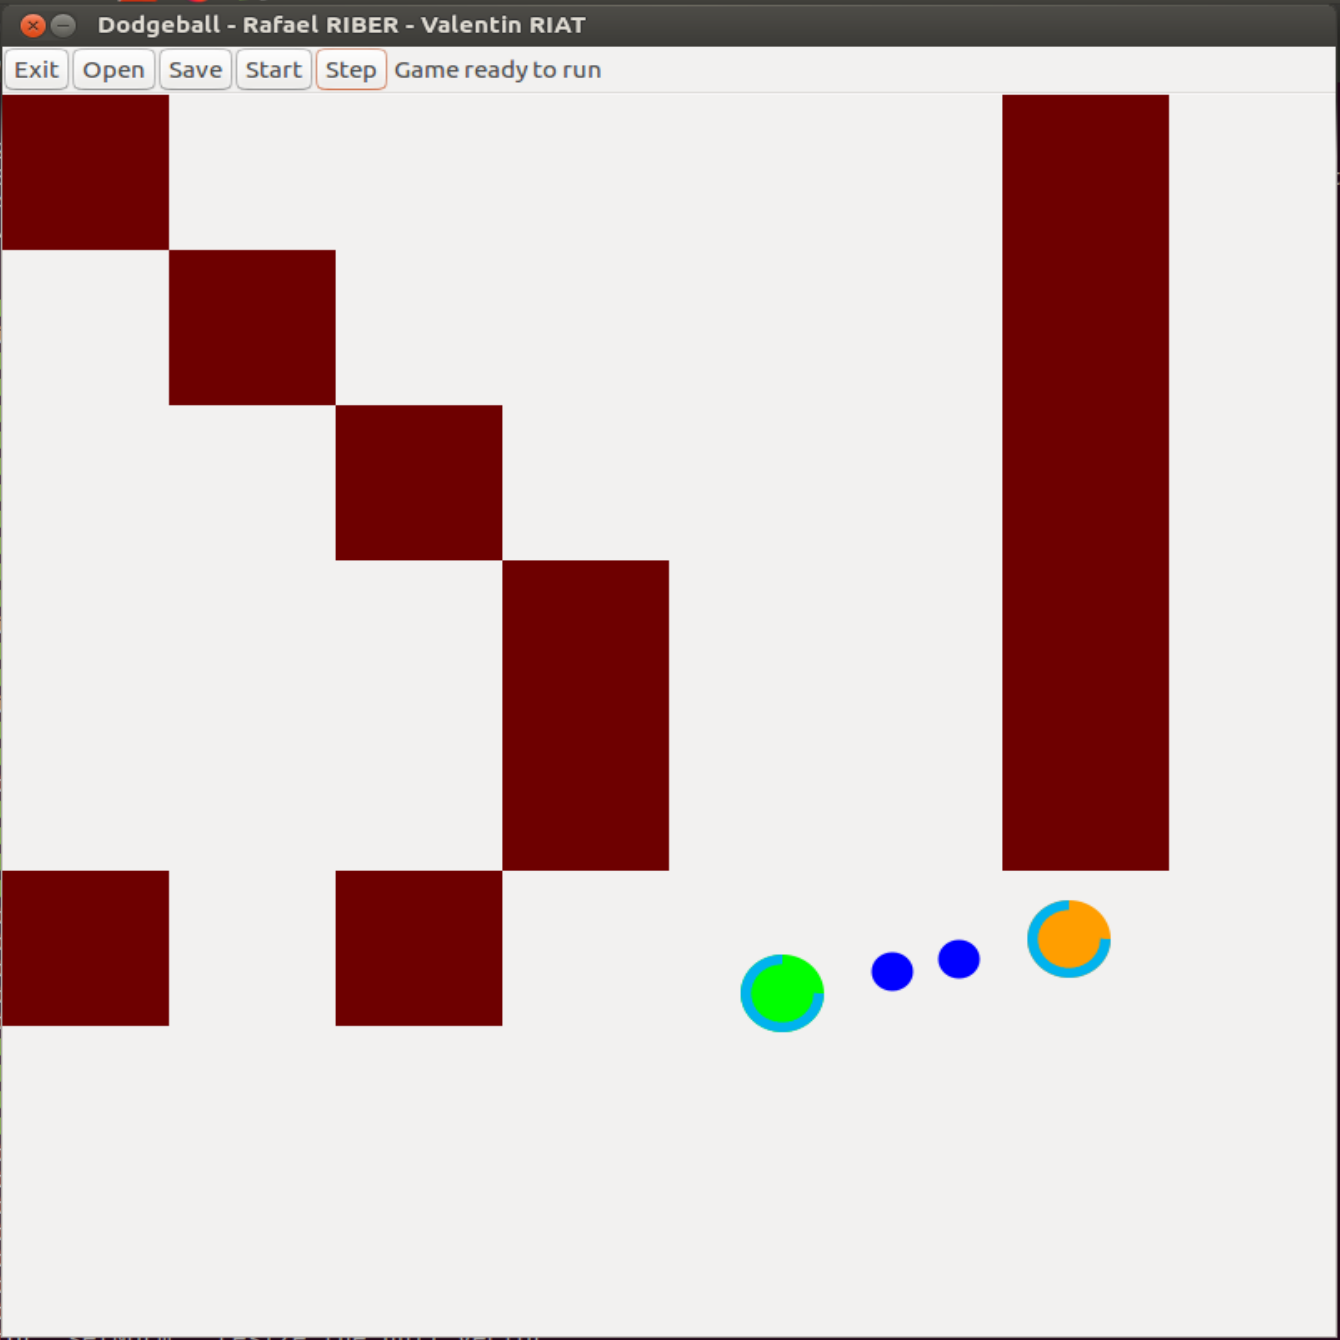
\includegraphics[width=\textwidth]{figures/sim8.PNG}
\end{minipage}
\begin{minipage}{0.33333333\textwidth}
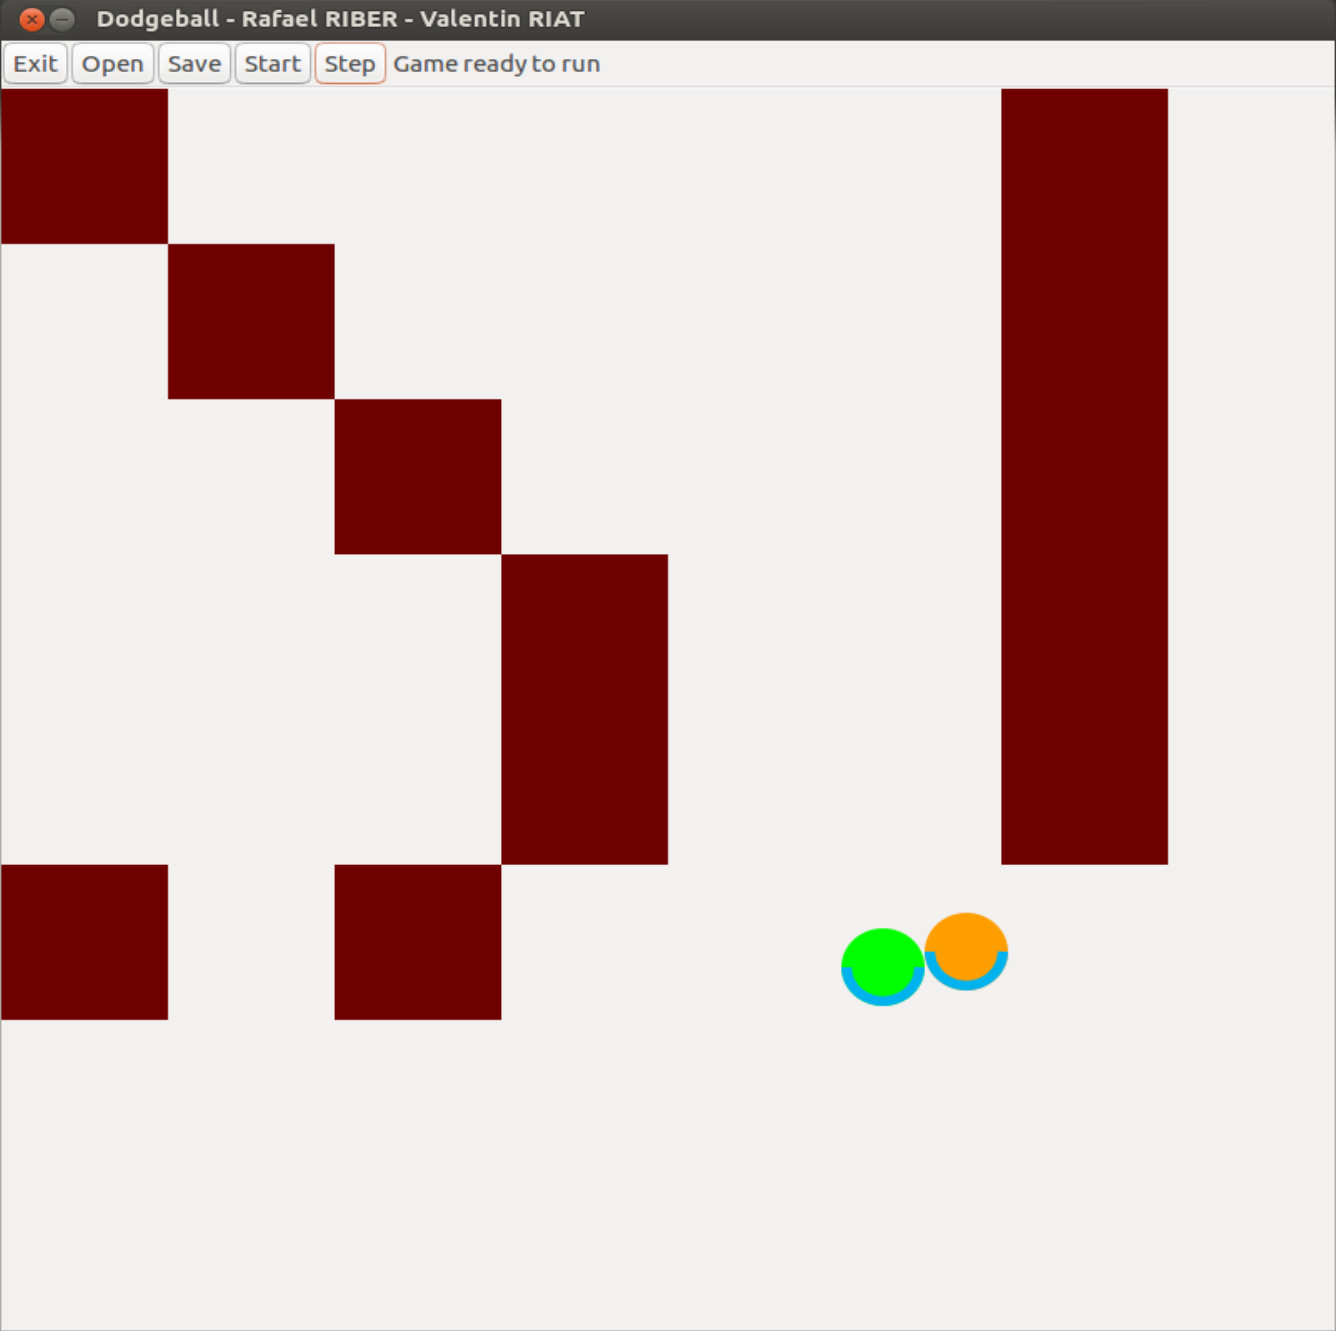
\includegraphics[width=\textwidth]{figures/sim9.PNG}
\end{minipage}
\begin{minipage}{0.33333333\textwidth}
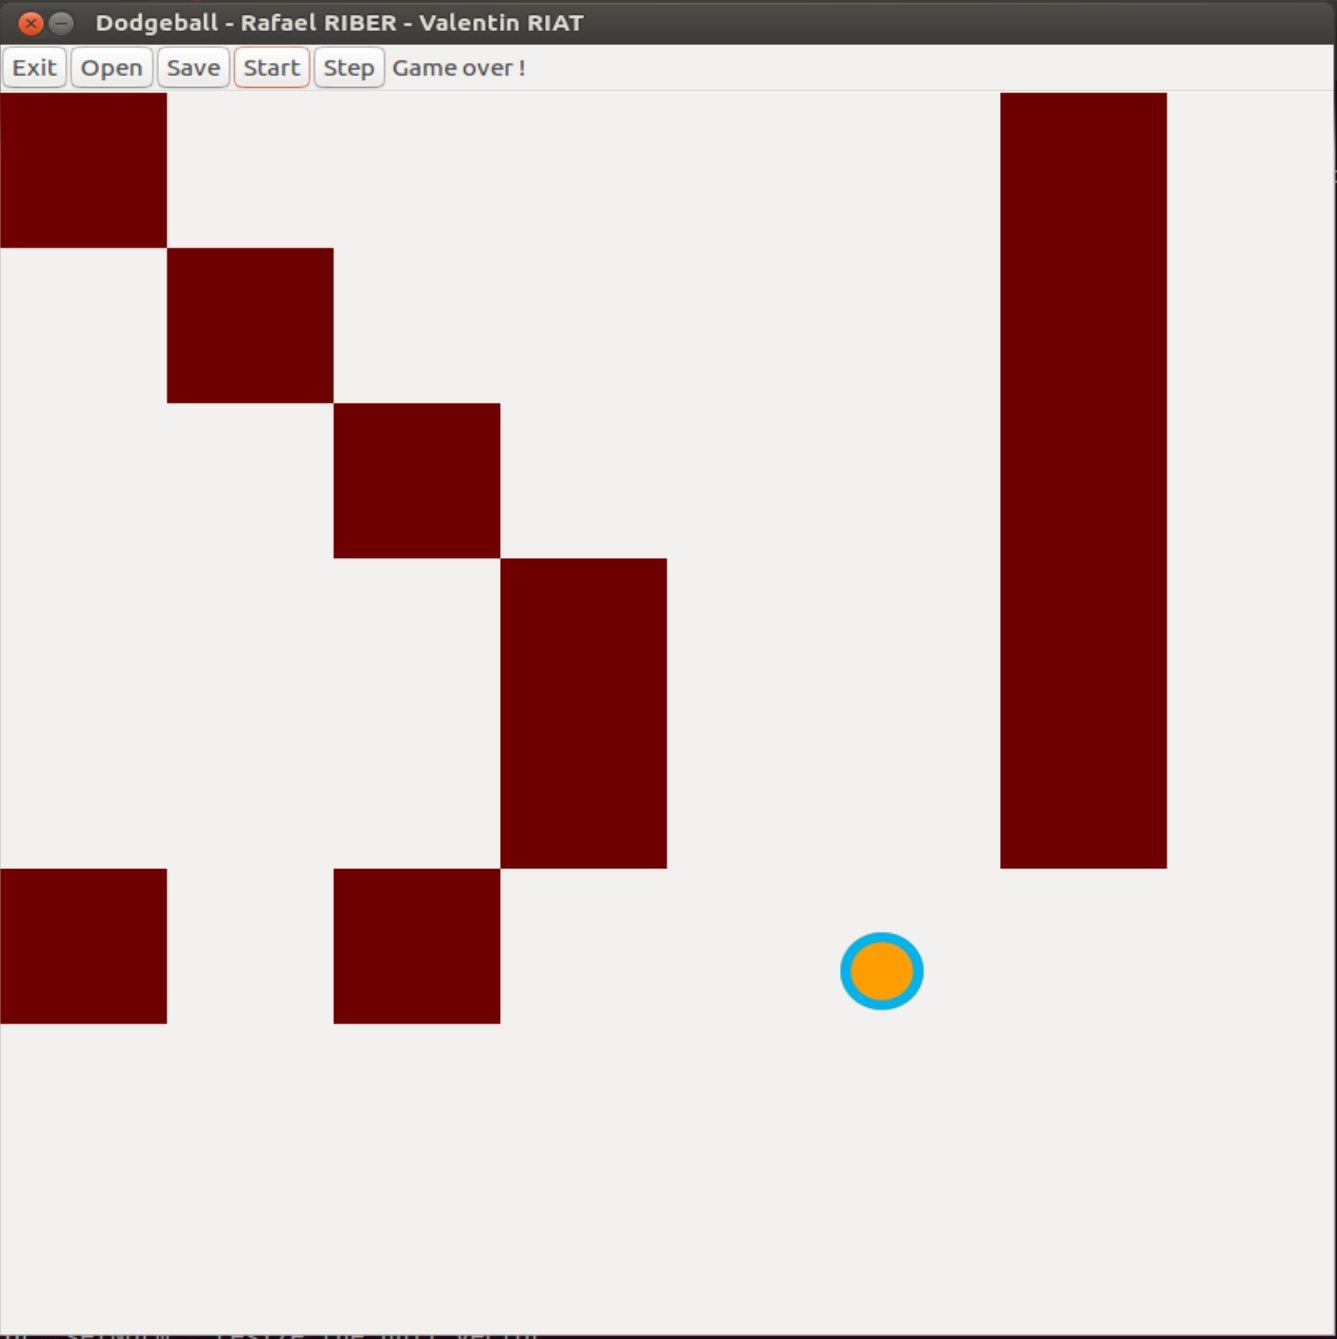
\includegraphics[width=\textwidth]{figures/sim10.PNG}
\end{minipage}

\section{Méthodologie}

Nous avons géré le code à l'aide d'un dépot GitHub privé, en créant des branches pour chaque nouvelle fonctionnalité ajoutée. Cette méthode nous a permis de travailler simultanément sans soucis de versions de fichiers, et de suivre chaque modification du code, en testant chaque nouvelle fonctionnalité sans modifier la branche principale avant que la fonctionnalité soit prête à être implémentée.

Nous avons commencé par le module Simulation, en implémentant l'automate de lecture. La gestion de code par Git nous a permis de travailler chacun sur chaque module, avec toutefois une focalisation de Valentin sur la simulation et de Rafael sur l'implémentation du GUI.

Le bug qui nous a posé le plus de problèmes à été l'automate de lecture qui sautait des lignes, et que nous avons du réécrire complètement afin d'arriver à une lecture correcte des fichiers de configuration.

\section{Conclusion}

Si nous devions refaire ce travail, nous aurions probablement ajouté plus de modules, afin de séparer les différentes tâches de simulation, par exemple. L'environnement mis à notre disposition nous a permis d'avoir des réponses rapides à nos questions, mais la machine virtuelle a parfois été difficile à utiliser du fait de sa lenteur.

\end{document}